\subsection{Kommunikasjon}
%Kommunikasjon, roller og normer, personligheter

%Hvordan gruppa har snakket med hverandre. Informasjonsflyt. Hvem sier hva. Initiativ. Kommunikasjonsmønster. Hvordan formidler vi kommunikasjon til hverandre? Er vi flinke til å være tydelig og oppklarende, eller bygger vi på antagelser og egne tolkninger? Hvilke roller har de forskjellige medlemmene i gruppa. Er de formet av oss selv eller faget og rammene vi har gitt oss? Faglig nivåforskjell/hetrogenitet/forkunnskaper.

God kommunikasjon er en av de viktigste karakteristikkene ved et effektivt team.
Dersom man skal klare å jobbe godt sammen for å levere et produkt kreves blant annet utveksling av kunnskap og diskusjoner om viktige valg.
I gruppen har kommunikasjonsmønstret utviklet seg fra start til slutt.
Gjennom flere ulike øvelser og felles arbeid har gruppen fått testet seg, fått tilbakemeldinger og muligheter til å foreta aktive endringer i hvordan gruppemedlemmene kommuniserer med hverandre.
\\

\subsubsection{Kommunikasjonsdynamikk}

Trenden med at medlemmene i gruppen hadde ulik mengde initiativ i diskusjoner var grunnlag for regel \#11 i samarbeidsavtalen: \textit{Alle i gruppen skal vise hverandre respekt.
Dette gjennom å lytte, bidra med egne meninger, gi konstruktiv kritikk og bygge videre på andres id\'{e}er.} 
Gruppen består av medlemmer som opprinnelig hadde veldig ulike \textit{tilnærminger} til åpne diskusjoner og samtaler.
For eksempel sier både Karsten og Jonas at de er klar over at de tar mye initiativ og \textit{tar stor plass} i diskusjoner.
Derimot forholder Simen og Ingelin seg forholdsvis stille, og tar gjerne ikke ordet like ofte.
Anna og Martin plasserer seg omtrent midt mellom de to andre \textit{grupperingene}.
Dette mønsteret i kommunikasjonen er noe gruppen var klar over ganske tidlig, og har jobbet med i løpet av prosjektperioden.
Som Jonas skriver i refleksjonen om hva han lærte om gruppen i løpet av 2. landsbydag:
\textit{"Vi har veldig ulike bakgrunner, både sosialt og faglig. Likevel virker alle åpne. Det er flere av oss som liker å ta ordet. Det er en bra start, men vi må være obs. på at alle får sagt det de ønsker."}
En aksjon for å oppnå punkt \#11 var å la ordet gå på rundgang når viktige avgjørelser skulle tas eller viktige temaer skulle diskuteres.
Slik fikk alle medlemmene muligheten til å legge frem sitt synspunkt, samt "tvunget" til å ha en mening om alt som ble diskutert.
Fordelen med dette er at ingen av gruppemedlemmene fikk muligheten til å "melde seg ut" av diskusjonene. \\

For å kontrollere at \#11 i samarbeidsavtalen ble overholdt ble punkt \#10 lagt til: \textit{Gruppen skal ha rullerende møteleder og sekretær for hver landsbydag. Møteleder har hovedansvar for å overse arbeidsplan og trivsel samt å være ordstyrer.}
Ordstyreren hadde som oppgave å fordele taletid mellom alle medlemmene i gruppen, og eventuelt oppmuntre medlemmer som hadde vært stille en stund.
Ordstyreren fikk fullmakt til å avbryte andre gruppemedlemmer når han/hun følte at dette var nødvendig.
Det kan likevel være utfordrende for ordstyrer å henge med på hvem som vil komme med innspill til hva i diskusjoner, spesielt når de fleste gruppemedlemmene hadde meninger om saken.
Jonas, som hadde erfaring med samarbeid fra tidligere, nevnte tidlig i prosjektet at innføring av møtetegn kunne være en god id\i{e} om diskusjonene ble for "kaotisk".
Selv om dette ikke ble brukt metodisk, var det tidvis i bruk.
Simen, som ikke er så flink å "presse seg inn" i diskusjonen, skiver for eksempel i refleksjonen fra 3. landsbydag: \textit{"Brukte møtetegn i dag og etter litt tid fikk jeg ordet, og alle fulgte med. Dette kan være fordi gruppen passer på å gi plass til de som vil snakke. Dette var mer effektivt enn å prøve å bryte inn i diskusjonen."}
Gruppen føler at innføringen av ordningen med ordstyrer trolig førte til en mer åpen og flytende kommunikasjon.
Mot slutten av prosjektet, spesielt da gruppen møtte utenfor de fastsatte onsdagene, var ikke behovet for ordstyrer like stort lengere.
Kanskje hadde kommunikasjonsdynamikken "satt seg" ved dette tidspunktet og alle i gruppen var mer oppmerksom på å gi alle plass. \\



\subsubsection{Kunnskapsutveksling}
EiT legger opp til at alle medlemmene som jobber med prosjektet skal få et faglig utbytte.
Både innenfor sine egne fagområder og resten av gruppens.
For å oppnå dette ønsket gruppen at det skulle være lett å dele den kunnskapen de enkelte medlemmene satt inne med med fra før.
Så tidlig som 2. landsbydag utarbeidet gruppen en samarbeidskontrakt.
Målet var å oppnå en felles oppfatning innad i gruppen om hvordan gruppearbeidet skulle utføres.
I tillegg skulle den bestemme hvilke krav gruppens medlemmer kunne stille til hverandre.
Hovedemnene var leveranse, læring og trivsel.
Samarbeidsavtalen ligger i vedlegg \ref{Ved:samarbeidsavtale}.
Viktigheten av god kommunikasjon innad i gruppen ble gjenspeilet i flere punkter i kontrakten.
\\
Et viktig poeng med EiT er tverrfaglig samarbeid. Dette målet ble reflektert i punkt 8 i samarbeidskontrakten: \textit{Gruppen skal drive kunnskapsutveksling gjennom diskusjon og drøfting av faglig innhold, samt utfordre hverandre til å gå utenfor den faglige komfortsonen.} Blant annet ville det være viktig å utnytte Ingelin sine kunnskaper om generell kjemi for at resten av gruppen skulle komme raskt igang med arbeidet.
Flere av gruppemedlemmene har vært takknemlig for hvor enkelt det har vært å spørre om andres kompetanse under prosjektarbeidet.
Karsten som har jobbet mye med de biologirettede delene av prosjektrapporten har gitt uttrykk for at Ingelin sine forhåndskunnskaper var til stor hjelp, og at Ingelin var villig til å avbryte eget arbeid for å hjelpe til.
Det er også av interesse å høre hva de ulike gruppemedlemmene har av faglige lidenskaper for å kunne skape et godt sosialt og løsningsorientert miljø i gruppen.
\\
Kommunikasjon er ikke bare muntlig kunnskapsutveksling, ei heller formelt nødvendigvis.
Et eksempel på hvordan dette har foregått er de tekniske løsningene rundt dokumentdeling og ferdigstilling av prosjekt- og prosessrapporten.
For å legge til rette for individuelt arbeid valgte gruppen å bruke en programvare som heter Git.
Dette programmet sørger for versjonskontroll og at dokumentene ble delte samt oppdaterte.
Programvaren tok litt tid å sette opp, men etter dette har medlemmene kunnet skrive selvstendig samtidig som det ikke var behov for å bekymre seg for at noen andres arbeid ble slettet i prosessen.
Ferdigstillingen av rapportene har blitt gjort i \LaTeX.
Begge disse tekniske løsningene har hatt noen implementeringsutfordringer som Jonas og Martin har jobbet med underveis.
Det har krevd at de begge bidro med å dele sin forhåndskunnskap og samarbeide om å finne ny informasjon som kunne belyse problemer som oppstod underveis.
\\
Siden samarbeidsavtalen var noe som ble utviklet tidlig, og før prosjektarbeidet hadde kommet skikkelig i gang, er det vanskelig å se om dette punktet har ført til noen vesentlig utvikling i gruppen.
Likevel viser dette seg å være en av flere årsaker til åpen kommunikasjon i gruppen.
\\

\subsubsection{Semantisk støy}

Øvelsen SITRA gikk ut på at gruppemedlemmene leste to fiktive refleksjoner av en og samme situasjon.
Medlemmene skulle først individuelt kategorisere setningene som situasjon, refleksjon, aksjon eller teori.
Deretter skulle tolkningene sammenlignes og diskuteres felles i gruppen.
Denne øvelsen trente gruppemedlemmene i kommunikasjon, og da spesielt i problemene som oppstår ved semantisk støy.
Semantisk støy handler om hvordan ord og uttrykk blir tolket.
Til å begynne med var det store ulikheter i oppfatningene av hva som hørte til i hver kategori.
Det krevdes derfor diskusjon og presisjon fra hvert medlem om hvor skillet mellom de ulike kategoriene skulle være.
Øvelsen viste hvor viktig det er å forklare andre medlemmer hva som menes med ulike begreper. 
Dette faktum er også tydeliggjort i \textit{Roger Schwarz} sine \textit{Grunnregler for effektive grupper}\cite{schwarz}. 
Han poengterer viktigheten av å sjekke antagelser og slutninger som trekkes fra det andre presenterer til deg.
\\
Det trekkes flere slutninger daglig, ofte automatisk og uten å være gjennomtenkt. 
Uten å være klar over det, kan slutningene oppfattes som fakta.
Dermed kan misforståelser oppstå, ved at deler av budskapet er blitt stengt ute eller mistolket.
Intensjonene til den andre kan dermed tolkes feilaktig i forhold til personens egentlige budskap.
Et utsagn kan tolkes på flere måter av mottakeren.
Mottakeren spør heller ikke alltid om budskapet er forstått riktig, men heller feiltolker.
Det kan derfor være til hjelp om den som kommer med utsagnet også utdyper det på eget initiativ.
Hvis det er tvil om intensjoner og budskap, må medlemmene ikke nøle med å spørre om alt er forstått korrekt.
Ved hjelp av SITRA-øvelsen ble gruppen for første gang introdusert for viktigheten av å presisere hva som legges i begreper.
\\
Under grupperefleksjonen landsbydag syv, diskuterte Anna og Karsten oppgavene til referentsrollen.
Begge tolket hverandres synspunkter for fort uten å ha forstått den andres egentlige budskap.
Det resulterte i at de trodde den andre hadde motsatte intensjoner, mens de faktisk hadde veldig like synspunkt om hva referenten hadde som oppgave. 
For utenom problemer med å formulere et synspunkt på en forståelig måte, innrømte flere av gruppemedlemmene at mangel på tålmodighet kunne føre til at slutninger ble trukket før et helt resonement har blitt lagt frem. 
Karsten ytret: \emph{"Min utfordring i forhold til disse grunnreglene, er at jeg har en tendens til å avbryte, ta ordet og trekke egne konklusjoner på andres innspill. Jeg har en tendens til å være utålmodig når andre bruker lang tid til å komme til saken."}
Etter å ha oppdaget hvor lett det er å misforstå andre, prøvde gruppen å hyppig stille spørsmål for å sikre at budskapet hadde blitt forstått riktig.
Å totalt utelukke at medlemmer trekker sine egne konklusjoner, vil alltid forekomme i en eller annen grad.
Ved å bli gjort direkte oppmerksom på situasjonen, kunne gruppen prøve å redusere omfanget av den videre i samarbeidet.
 \\
Et annet tiltak for å redusere semantisk støy er å eksemplifisere forklaringer.
Dette gjør det lettere for motparten å validere utsagnene, siden eksemplene gjerne henviser til observerte eller observerbare data.
Dette bør gjerne brukes for å tydeliggjøre sentrale begreper, da det er viktig for å få en felles oppfattelse av disse så tidlig som mulig.
Simen var svært flink til å tegne for å illustrere sine idéer slik at alle gruppemedlemmene fikk et klart bilde av hva de innebar.
\\
En uenighet mellom to personer kan fort havne i en posisjonsorientert og låst situasjon.
Partene kan mene at de selv har rett, uansett hvilke beviser som måtte foreligge.
For å finne måter å sjekke misforståelser, må det bli enighet om hva problemet omfatter. Begge parter kan ha tatt hensyn til hver sine aspekter.
Videre må det diskuteres om begge samtidig kan ha rett.
Et mer gjennomgående og ikke-iscenesatt eksempel på dette er at Anna og Karsten ikke har norsk som morsmål.
Dette har aldri skapt store misforståelser i gruppen, sannsynligvis fordi Anna har vært tydelig fra starten av om at norsken hennes ikke er perfekt.
Landsbydag syv gjentok Anna under grupperefleksjonen: \emph{"Jeg vil gjenta at siden jeg har en språkbarriere vil jeg jobbe for å være enda tydeligere og presis når jeg formulerer mine idéer"}.
\\
Disse grunnreglene og andre øvelser, har gjort at gruppen har vært flink til å formulere seg, og ikke minst få og spørre om bekreftelse på at innholdet er forstått korrekt.
Gruppen er fortsatt ydmyk og fullt klar over at det finnes et forbedringspotensiale hos alle gruppemedlemmene.
\\

%\subsubsection{Grunnregler for effektive grupper}

En øvelse som ble gjennomgått i gruppa var å diskutere et sett med regler hver enkelt kan følge for å oppnå effektivt gruppearbeid.
Dette ble gjort for at samtlige gruppemedlemmer tidlig i prosjektet skulle bli mer bevisste på hvordan man kan forholde seg for å unngå kommunikasjonsproblemer.
Reglene beskriver visse adferder som er med på å gjøre kommunikasjon i en gruppe mer tydelig \cite{schwarz}:

%\paragraph{Sjekk antakelser og slutninger}


%\paragraph{Del all relevant informasjon}
%Om ikke all relevant informasjon foreligger, vil gruppas kollektive misforståelse av et emne kunne bidra til å ta feil beslutninger.

\paragraph{Eksemplifiser og bli enige om viktige begreper}


\paragraph{Forklar ditt resonnement og din intensjon}\label{forklardittres}

%\paragraph{Fokus på interesser, ikke posisjon}\label{interpos}
%Når et fellesskap skal komme til enighet hender det at noen er tidlig ute med et forslag til løsning.
%Da stiller vedkommende seg i en posisjon hvor det er ukjent for de andre hvilke interesser denne personen legger til grunn for en slik løsning.
%Problemet er at slike forslag og motforslag kan være inkompatible selv om interessene egentlig stemmer overens.
%Hvis man åpner med å dele interesser med de andre, er det lettere å utarbeide løsninger i fellesskap.
%Om andre tidlig kommer med løsninger istedet for å begrunne dem, kan man spørre om interessene som ligger til grunn.

\paragraph{Kombiner sakføring og granskning}
Diskusjoner kan noen ganger arte seg slik at man snakker forbi hverandre.
For å unngå dette, kan man invitere motparten til å granske ens egne utsagn, gjerne med å stille oppfølgingsspørsmål.
Dette virker sakførende, siden det bidrar til en felles forståelse av saken mellom partene.
Retoriske spørsmål vil kunne virke sakførende, men ikke granskende, da det kan få motparten til å bli defensiv og holde tilbake informasjon.
Grunnen til at man bør granske, er at man kan avklare om motparten har forskjellige antakelser eller baserer seg på annen informasjon enn en selv.

\paragraph{Finn måter for å sjekke misforståelser}


%\paragraph{Diskuter udiskutable emner}
%I grupper kan det være saker som påvirker gruppas oppgave, men som det er vanskelig å diskutere i fellesskap.
%Det er gjerne saker som skyldes et medlem, og man vegrer seg for å snakke med denne personen om det.
%Emnet holdes kanskje udiskutert, eller man tar det opp med andre i gruppa, noe som ikke løser problemet.
%Man kan gjøre gruppa oppmerksom på at man skal diskutere noe udiskutabelt.
%Alternativt kan man si ifra til den det gjelder at man kommer til å ta opp temaet i fellesskap.
%Det siste gir personen mulighet til å forsvare seg i diskusjonen som kommer, noe som vil virke mest mulig skånsomt.

%\paragraph{Bruk en beslutningsprosess for passe enighet}\label{beslutningsprosess}
%Selv om alle i en gruppe idéelt sett kunne vært enige, som når man har oppnådd konsensus, kan det være krevende eller umulig å oppnå.
%I en konsultativ beslutningsprosess tar lederen en avgjørelse etter at temaet er diskutert.
%For en delegativ beslutningsprosess gir lederen beslutningsoppgaven til en del av gruppen, gjerne gitt endel begrensninger.
%Noen gruppemedlemmer kan kreve å få viljen sin for å kunne utføre sin oppgave, og noen ganger er konsensus nødvendig.
%Man må avveie hvor stor grad av enighet som trengs i forhold til hvor mye som skal til for å oppnå dette.

\subsubsection{Trivsel kontra åpenhet}

Gruppen har alltid kommunisert på en inkluderende og høflig måte. 
Særlig i starten er det vanlig at samtaler er preget av forsiktig og overfladisk innhold. 
For at kommunikasjonen i en gruppe skal være svært direkte og åpen, kreves det oftest at medlemmene føler seg komfortable og kjent med resten av gruppen. 
En slik utvikling ble antydet i flere samarbeidsindikatorer. \\

Samarbeidsindikatoren baseres på en spørreundersøkelse som holdes tidlig, midtveis og sent i semesteret.
Hovedfokuset for samarbeidsindikatoren har vært å følge utviklingen av det sosiale samværet, samt diskutere hvilke effekter dette har hatt på gruppens produktive kapasitet.
Resultatet av undersøkelsen ble fremstilt i et diagram med fire akser: \textit{Ærlig og direkte}, \textit{forpliktet og tillitsfull}, \textit{effektiv og strukturert} og \textit{åpen og lyttende}.
Jo lengre vekk fra sentrum, jo bedre.
I forbindelse med kommunikasjon i gruppen, er punktet som kalles \textit{Ærlig og direkte} den viktigste. 
Uten ærlig og direkte kommunikasjon kan et gruppesamarbeid resultere i at ikke-tema (\textit{'Alle vet det' - ingen snakker om det)} oppstår.
Indikatorene er gitt i figur \ref{samind1}, \ref{samind2} og \ref{samind3}.

\begin{figure}[h!]
  \centering
    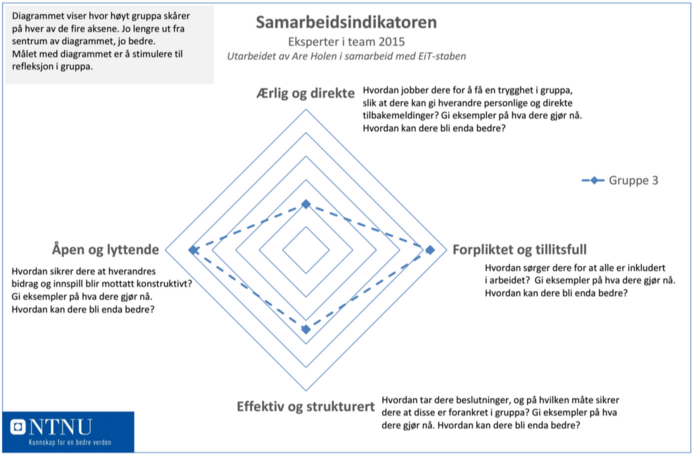
\includegraphics[width=0.5\textwidth]{Bilder/samarbeidsindikator1.png}
  \caption{Samarbeidsindikator 1 basert på undersøkelse landsbydag 5.}
    \label{samind1}
\end{figure}

Den første samarbeidsindikatoren, figur \ref{samind1}, antyder at gruppen ikke har vært tydelig nok når det gjelder ærlig og direkte tilbakemelding.
En naturlig årsak til at gruppen scoret lavt på ærlig og direkte, kan være at medlemmene ikke ønsket å ødelegge den positive stemningen.
Gruppen hadde samarbeidet i så kort tid at mottagelsen av direkte tilbakemeldinger og kritikk, fortsatt var ukjent.
Resultatet var ikke en stor overraskelse for gruppen, da få situasjoner som inneholdt kritikk av noe slag hadde oppstått.
Det ble enighet om at årsaken ikke var at gruppen og medlemmene ikke ville håndtere kritikk på en konstruktiv måte, men at utfallet var en naturlig følge av at samarbeidet var i en tidlig fase.
Indikatoren stimulerte likevel til at det å gi ærlig og direkte tilbakemelding, ble satt i fokus. \\

\begin{figure}[h!]
\centering
    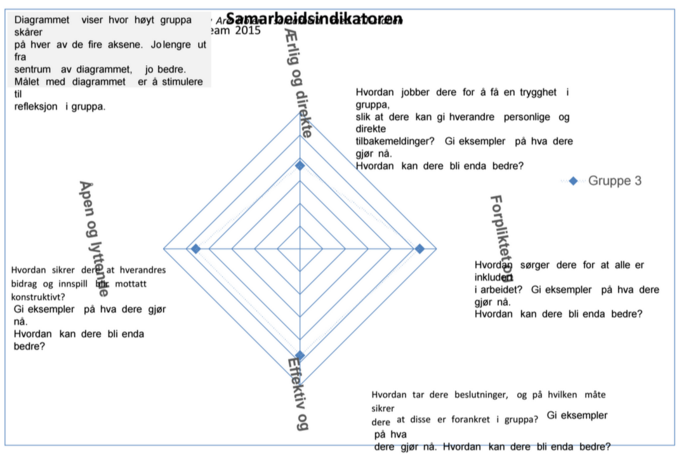
\includegraphics[width=0.5\textwidth]{Bilder/samarbeidsindikator_2.png}
 \caption{Samarbeidsindikator 2 basert på undersøkelse landsbydag 9.}
    \label{samind2}
\end{figure}

\begin{figure}[h!]
  \centering
    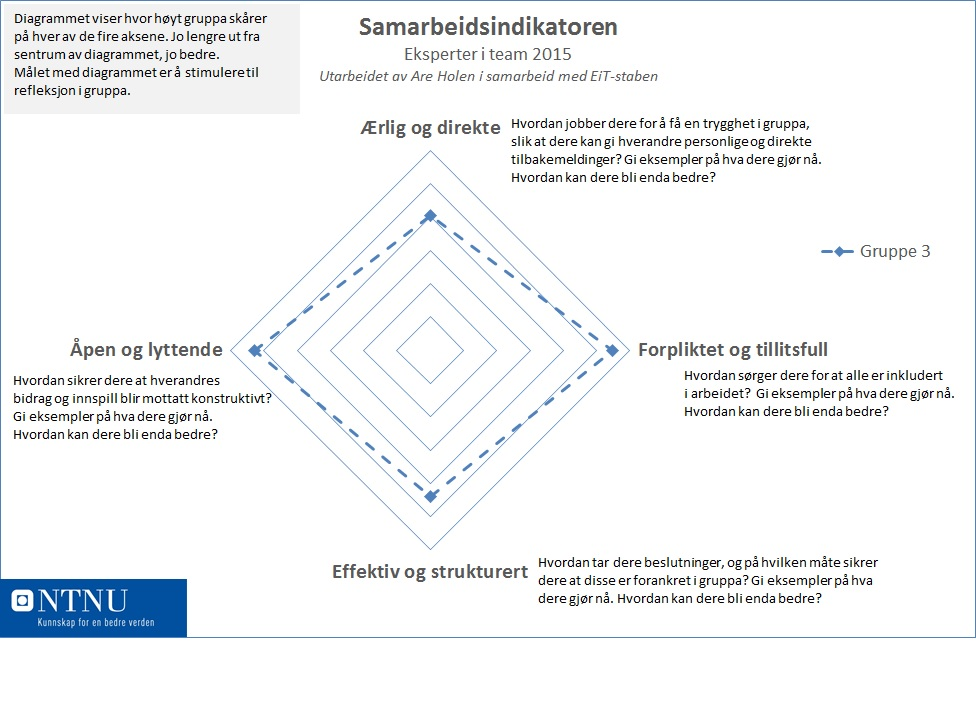
\includegraphics[width=0.5\textwidth]{Bilder/samarbeidsindikator_3.jpg}
    \caption{Samarbeidsindikator 3 basert på undersøkelse landsbydag 14.}
    \label{samind3}
\end{figure}

Gjennomgående for alle samarbeidsindikatorene var at gruppen scoret dårligst på vurderingskriteriet \textit{ærlig og direkte}. 
Utviklingen har likevel vært positiv, da de neste to indikatorene, figur \ref{samind2} og \ref{samind3}, viser forbedring (punktet har beveget seg vekk fra sentrum). 
Et konkret eksempel på å gi og få tilbakemelding fra medlemmene, var under grupperefleksjonen på slutten av dagen da de to som hadde hatt rolle som ordstyrer og referent, fikk direkte tilbakemelding.
Under refleksjonen landsbydag 6 sa Martin: \textit{"Simen mangler litt autoritet som ordstyrer. Kanskje han er for snill. Han kunne vært tydeligere på hvordan ting skulle blitt gjort, som for eksempel å innlede en 'runde rundt bordet'"}.
Slik tilbakemelding ga positive konsekvenser både for gruppen og for medlemmet som mottok den.
Neste gang Simen var ordstyrer var det tydelig at han hadde tatt kritikken til seg, og lært fra forrige gang.
Ved å gi tilbakemelding på en så konkret oppgave som ordstyrerrollen, ble terskelen også lavere ved andre situasjoner. \\

Som nevnt i starten, har gruppen alltid kommunisert på en høflig og positiv måte.
I starten skyldtes høfligheten at medlemmene kun kjente hverandre på en overfladisk måte, og at kommunikasjonen ble preget av dette.
I slutten av samarbeidet var kommunikasjonen fortsatt like positiv, men på helt annet grunnlag.
Medlemmene kunne gi positive og konkrete tilbakemeldinger på hverandres arbeid basert på at hver enkelts sterke sider hadde blitt avdekket.